\section{Software architecture and design}
\label{chapter2}

\paragraph
{}
When the ACC is activated, Node 2 executes a periodic task to receive distance measurements from Node 1. Based on these readings, it calculates the updated speed of the virtual car. In case of an alarm situation - such as invalid or missing sensor data, or a loss of Bluetooth communication - the ACC is automatically deactivated and the driver is alerted to take over control.

\subsection{Software modules}

\begin{itemize}
	\item CryptoComm component on Node 1 and Node 2
	\item CommThread (Tx) on Node 1
	\item SensorThread on Node 1
	\item CommThread (Rx) on Node 2
	\item ACCThread on Node 2
	\item MainWindow on Node 2
\end{itemize}

\subsubsection{Safety related modules}
\begin{enumerate}
	\item SensorThread: \\
		Description: Reads distance measurement from two redundant proximity sensors on Node 1\\
		Functions: void acc::SensorThread::threadLoop()\\
		Data: gCurrentDistanceReading (write)\\
		Requirements see: \ref{req.1}, \ref{req.2} \\
	\item CommThread (Node 1): \\
		Description: The communication thread on Node 1 sends distance readings, starts listening again if the Bluetooth connection is closed \\
		Functions: void acc::CommThread::threadLoop()\\
		Data: gCurrentDistanceReading (read)\\
		Requirements see: \ref{req.8} \\
	\item CommThread (Node 2): \\
		Description: The communication thread on Node 2 receives and validates distance readings, restarts broken Bluetooth connections \\
		Functions: void acc::CommThread::threadLoop()\\
		Data: gCurrentDistanceReading (write)\\
		Requirements see: \ref{req.8} \\
	\item ACCThread: \\
		Description: Processes received distance readings, turns ACC off if no valid readings are available and warns in case of an error \\
		Functions: acc::ACCThread::threadLoop()\\
		Data: gCurrentDistanceReading (read), gVehicleState(read, write)\\
		Requirements see: \ref{req.4}, \ref{req.5}, \ref{req.7}, \ref{req.11}, \ref{req.12}, \ref{req.13} \\
	\item MainWindow: \\
		Description: Informs the driver about vehicle speed, distance to the next car in front, status of the ACC \\
		Functions: void MainWindow::onSimTick()\\
		Data: gVehicleState(read, write) \\
		Requirements see: \ref{req.3}, \ref{req.6}, \ref{req.9}, \ref{req.10}, \ref{req.11} \\
\end{enumerate}

\subsubsection{Security related modules}

\begin{enumerate}
	\item CryptoComm: \\
		Description: Session Key generation, MAC generation and validation.; Sending and Receiving Bluetooth.\\
		Functions: TBD\\
		Data: TBD\\
		Requirements see: TBD\\
\end{enumerate}

\subsubsection{Modules with no influence on Safety and Security}

\begin{enumerate}
	\item Helper: \\
		Description: contains commonly used helper functions and classes \\
		Functions: TBD\\
		Data: TBD\\
		Requirements see: TBD\\
\end{enumerate}

\subsection{Libraries}

Description of used function with parameters.

\begin{enumerate}
	\item LibTomCrypt: \href{https://github.com/libtom/libtomcrypt.git} {https://github.com/libtom/libtomcrypt.git}, used for random number generation, AES session key generation, HMAC generation and verification.
	\item LibTomMath: \href{https://github.com/libtom/libtommath.git} {https://github.com/libtom/libtommath.git}, required by LibTomCrypt.
	\item pigpio: \href{https://github.com/joan2937/pigpio.git} {https://github.com/joan2937/pigpio.git}, used for accessing readings of ultrasonic sensors.
	\item catch2: \href{https://github.com/catchorg/Catch2.git} {https://github.com/catchorg/Catch2.git}, unit test framework
	\item glibc, libstdc++: Posix functions for timestamp retrieval, pthread creation, mutex creation, output stream handling, containers, e.g. std::array
	\item bluez, gio: Libraries for setting up Bluetooth sockets
\end{enumerate}

\subsection{Interrupts}

No interrupts, or interrupt service routines are used in this project.

\subsection{Pinout}

In this subsection, the pinouts are presented separately for Node 1 and Node 2. Since both Nodes are based on a Raspberry Pi, the following diagram \ref{fig:raspi} shows the general pinout configuration of the Raspberry Pi.

\begin{figure}[h]
	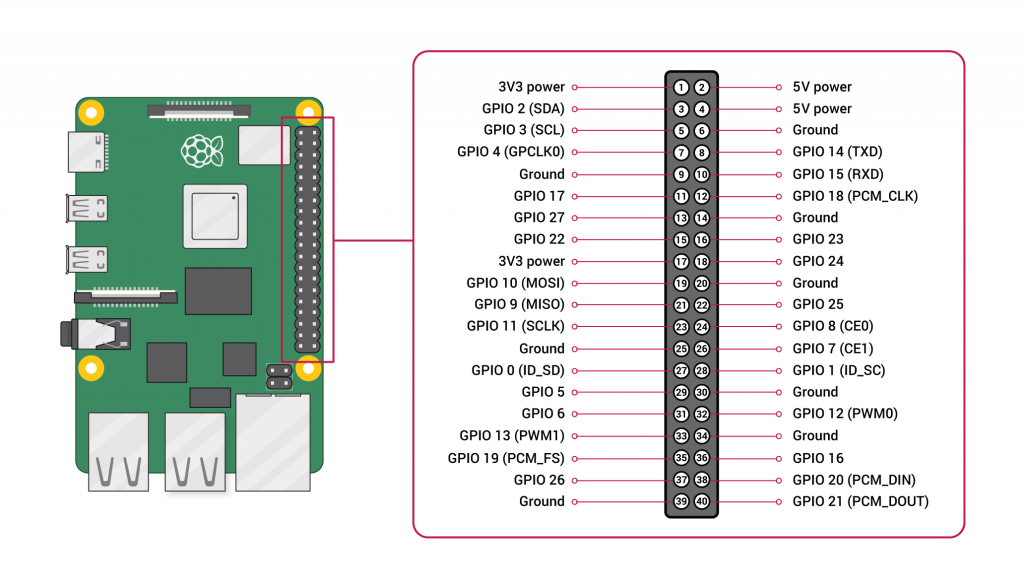
\includegraphics[height=50mm]{images/GPIO-Pinout-Diagram-2.png}
	\centering
	\caption{Raspberry Pi pinout configuration from \href{https://prilchen.de/raspberry-pis-gpio-ein-tor-zu-unzaehligen-projekten/} {prilchen.de}}
	\label{fig:raspi}
\end{figure}

\subsubsection{Node 1}

For Node 1, two ultrasonic sensors (HC-SR04) are connected to the Raspberry Pi. 
The VCC pin of each sensor is connected to a 5V power pin, while the GND of both sensors is connected to ground on the Raspberry Pi.
The TRIG pins are wired to GPIO 17 and 18, and the ECHO pins are connected to GPIO 23 and 24 through
 a voltage divider using two resistors ($R_1 = 1000\,\Omega$ and $R_2 = 2000\,\Omega$) to safely reduce the 
 signal from 5V to 3.3V. 
}

\subsubsection{Node 2}

For Node 2, the Raspberry Pi 4 is connected to the Raspberry Pi 7-inch Touch Display.  
The flat DSI ribbon cable is used to transmit the video signal and touch interface, while the four jumper wires provide power and enable I²C communication between the Raspberry Pi and the display controller. The wiring is as follows:

\begin{itemize}
    \item The \textbf{5V pin} of the display (marked ``5V'') is connected to the \textbf{5V power pin} of the Raspberry Pi (pin~4 on the GPIO header) \emph{(red cable)}.
    \item The \textbf{GND pin} of the display (marked ``GND'') is connected to the \textbf{ground pin} of the Raspberry Pi (pin~6 on the GPIO header) \emph{(black cable)}.
    \item The \textbf{SCL pin} of the display is connected to the \textbf{SCL pin} of the Raspberry Pi (pin~5 / GPIO~3) \emph{(yellow cable)}.
    \item The \textbf{SDA pin} of the display is connected to the \textbf{SDA pin} of the Raspberry Pi (pin~3 / GPIO~2) \emph{(green cable)}.
\end{itemize}

The wiring can be seen in Figure \ref{fig:node2-raspy} and \ref{fig:node2-display}.

\begin{figure}[h]
	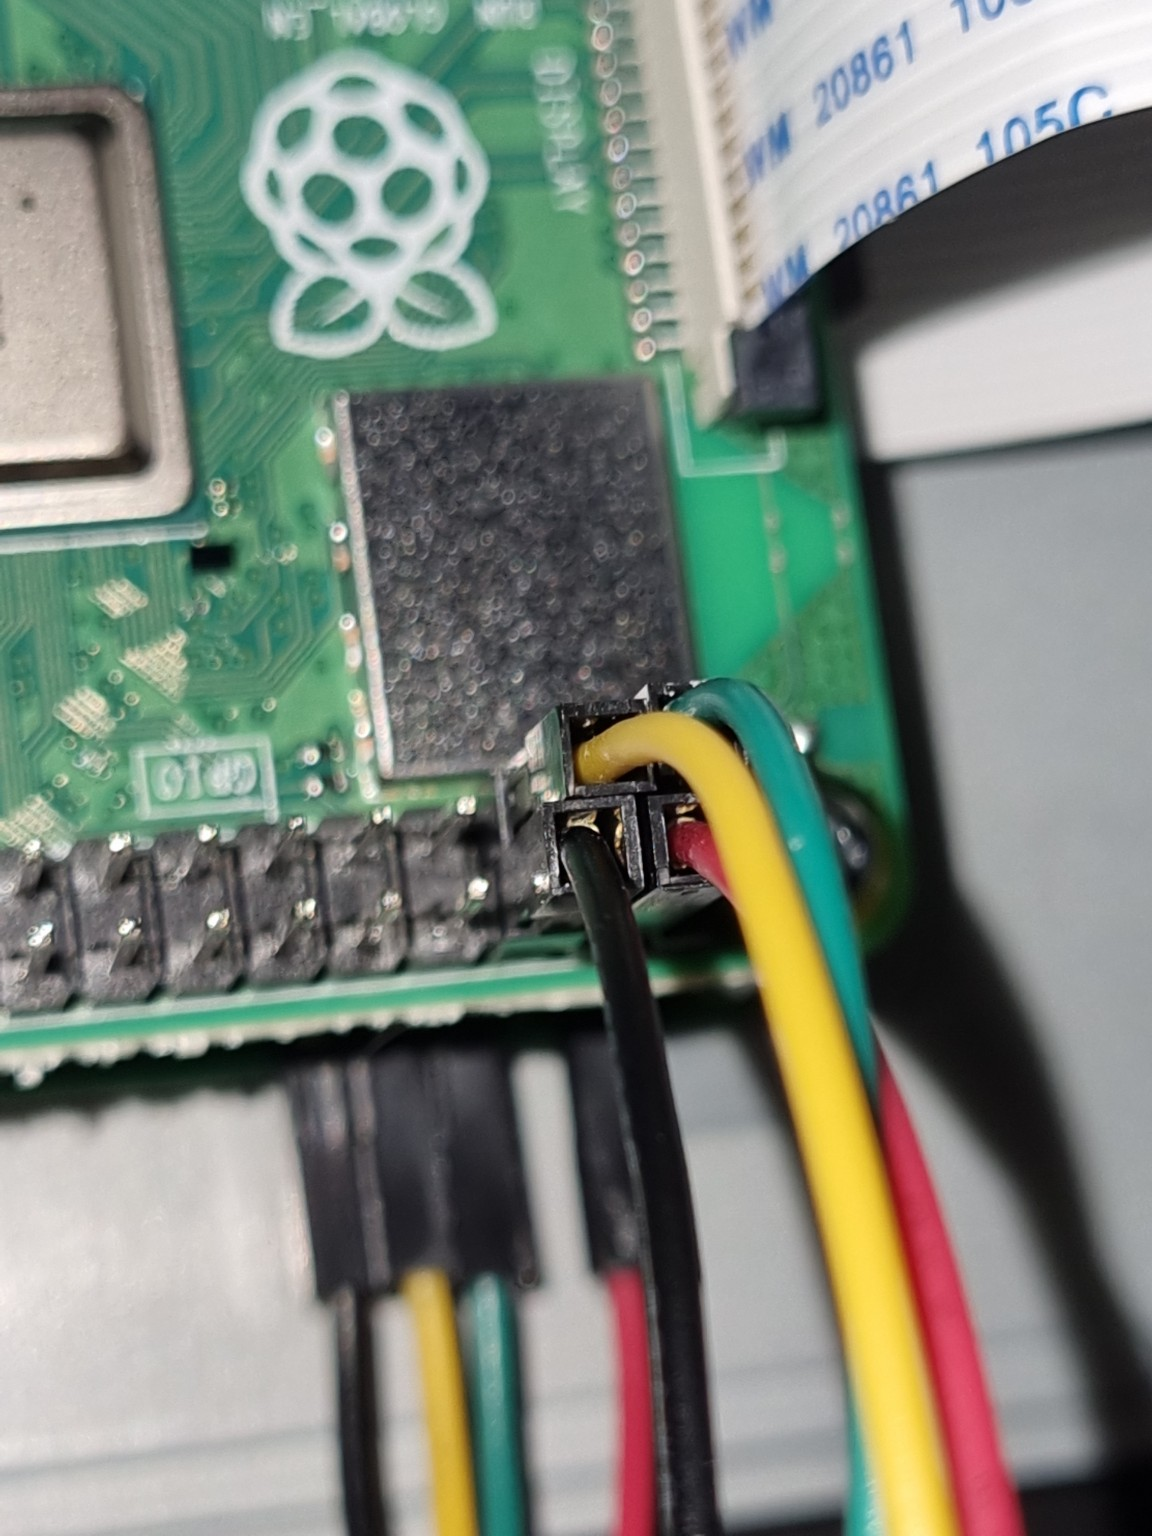
\includegraphics[height=100mm]{images/node2-raspy.jpg}
	\centering
	\caption{Pinout Node 2 Raspberry Pi}
	\label{fig:node2-raspy}
\end{figure}

\begin{figure}[h]
	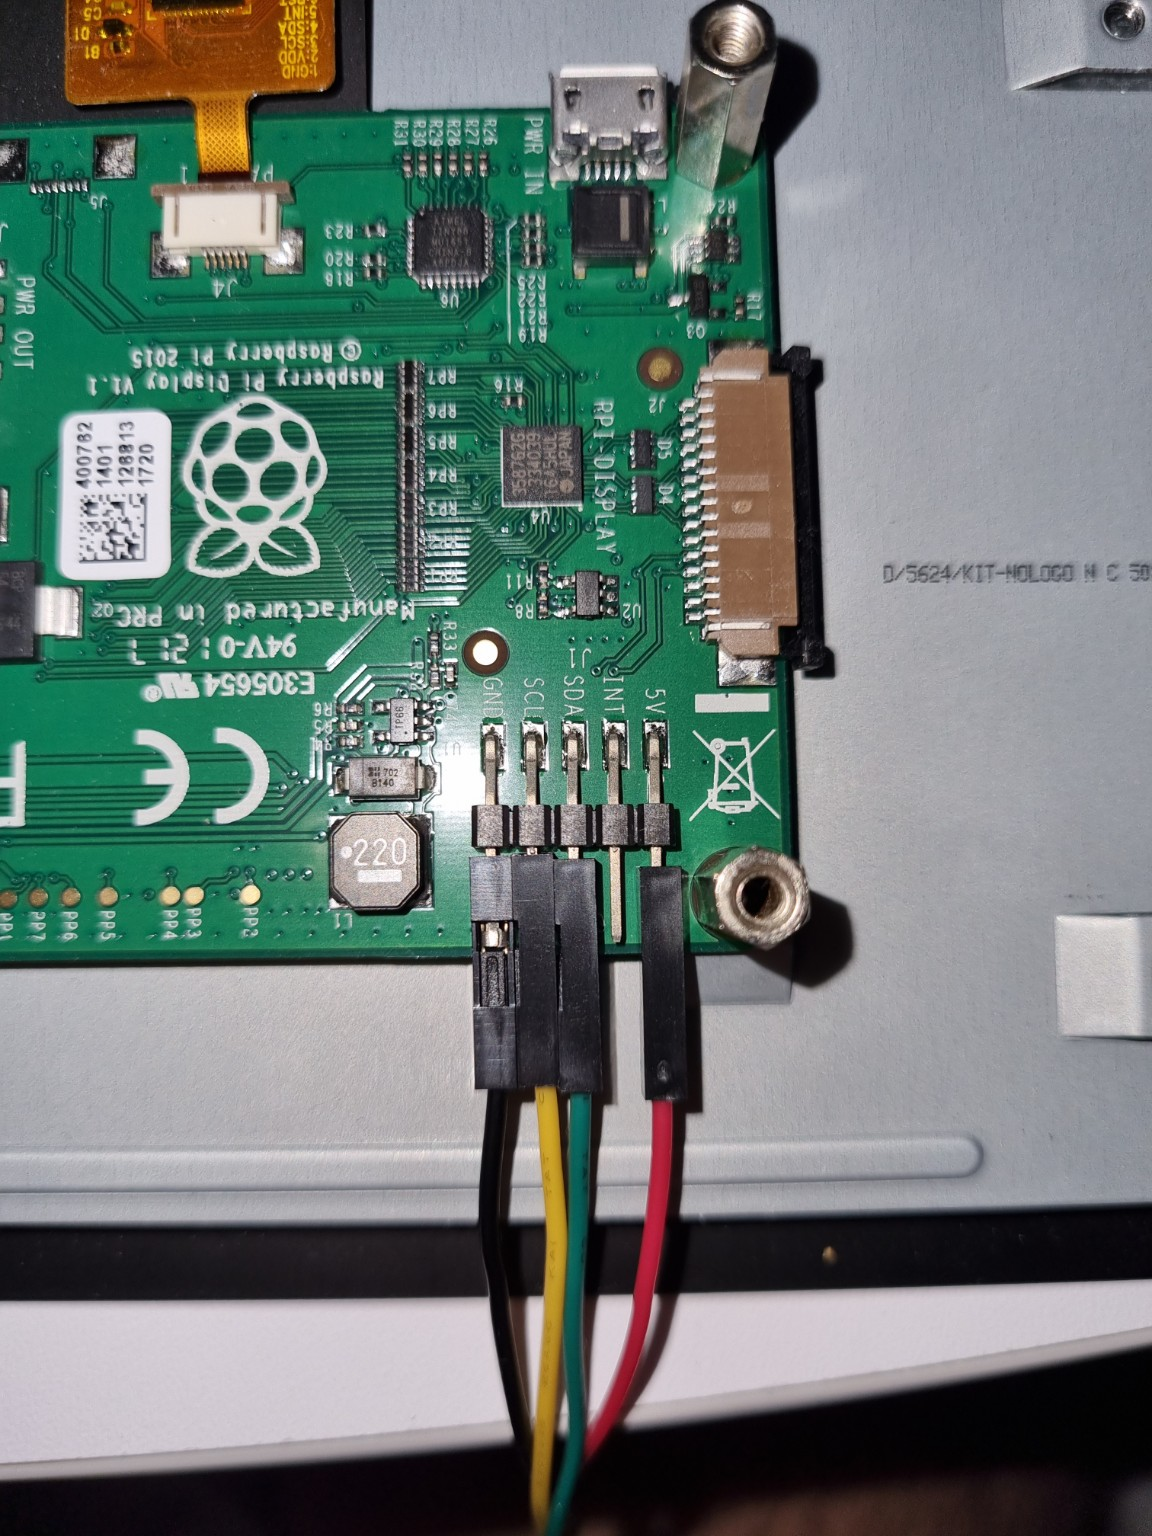
\includegraphics[height=100mm]{images/node2-display.jpg}
	\centering
	\caption{Pinout Node 2 Display}
	\label{fig:node2-display}
\end{figure}

\clearpage
\subsection{GUI}

Figure \ref{fig:gui} shows the dashboard GUI, containing the controls for accelerating and decelerating the vehicle, and for activating adaptive cruise control. It also contains elements showing the vehicles current speed, the distance to the nearest object in front of the car, and the status of the ACC system.

\begin{figure}[h]
	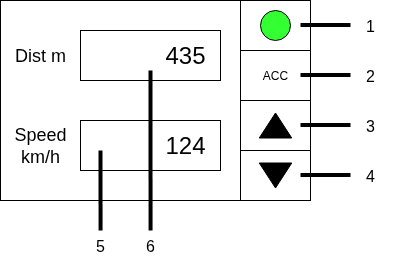
\includegraphics[height=50mm]{images/GUI.png}
	\centering
	\caption{Dashboard GUI}
	\label{fig:gui}
\end{figure}

\begin{enumerate}
  \item ACC Status LED: Shows the status of the ACC system, green if it is in an operational state, red, if ACC  is in a failed state.
  \item ACC Button: Push Button to activate ACC. Can only be pushed if ACC is in operational state.
  \item Accelerate Button: Increases the vehicle speed by 5 km/h (up to 200 km/h), deactivates ACC, if it was active.
  \item Decelerate Button: Decreases the vehicle speed by 5 km/h (down to 0 km/h), deactivates ACC, if it was active.
  \item Speed Display: Shows current vehicle speed
  \item Distance Display: Shows distance of the nearest object in front of the vehicle, does not display anything if ACC is in failed state.
\end{enumerate}

\subsection{Communication}

\paragraph{} Immediately after the communication is set up, Node 1 and Node 2 exchange 32 byte random numbers. These two numbers and a 32 byte pre-shared key are concatenated and put into a key derivation function returning a 256 bit AES session key used for HMAC generation. The message layout for these messages is shown in the first message in Figure \ref{fig:msg}.

\paragraph{}The messages which Node 1 and Node 2 are exchanging contain two fields:
\begin{itemize}
	\item MessageType: 1 byte, set to zero
	\item Random: 32 bytes, a random number generated by the sender node
\end{itemize}

FIXME: After key establishment, we should use a challenge-response round, so each participant proves to the other it owns the PSK. If that does not work on both sides, the connection should be dropped.

\paragraph{} After the common session key is established, Node 1 periodically sends sensor messages to Node 2. The message layout looks like depicted in the second entry in Figure \ref{fig:msg}. All multi byte fields are encoded as big-endian/in network byte order, i.e. the first byte of a field contains the MSB.

\paragraph{} The message has the following layout:
\begin{itemize}
	\item MessageType: 1 byte, indicates the content of the Payload field
	\item Counter: 4 bytes, zero based 32 bit unsigned integer
	\item Payload: Holds the transmitted information
	\item HMAC: SHA-256 based HMAC, protecting all fields before the HMAC
\end{itemize}

\paragraph{} The sensor message, sent from Node 1 to Node 2, holds the \emph{Distance} field, conveying the most recent distance readings from Node1. In the error free case, that field holds values in the range of [0..400] indicating the measured distance to the next object in [m]. A value of \emph{0} indicates a measured distance below one meter, while a value of \emph{400} indicates a distance of 400 meters or a greater distance. A value of \emph{0xffff} indicates that both sensors yielded inconsistent readings (i.e. readings deviating by more than 10\%), and the value of \emph{0xfffe} indicates that Node 1 detected a failure of one or both proximity sensors.

\begin{figure}[h]
	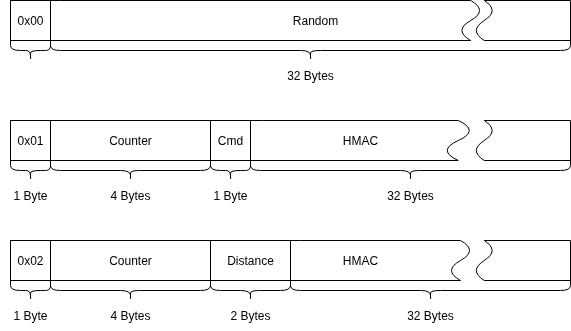
\includegraphics[height=50mm]{images/MessageLayout.png}
	\centering
	\caption{Layout of Messages}
	\label{fig:msg}
\end{figure}
